%% Vorlage: https://sdq.kastel.kit.edu/wiki/Dokumentvorlagen

\documentclass{sdqbeamer}[smallfoot]

\groupname{Artificial Intelligence for Language Technologies}
\grouplogo{}

\title[Campus Plan Bot]{Campus Plan Bot}
\subtitle{Practical: Natural Language Dialogue Modeling}
\author[Marwitz, Schittny]{Thomas Marwitz and Frederik Schittny}

\date[23.\,7.\,2025]{23. July 2025}

\usepackage{lipsum}
\usepackage{graphicx}

\begin{document}

%Titelseite
\begin{frame}[title white horizontal, picture=images/campusplan_cover, kitlogo=black]
\titlepage
\end{frame}

%Inhaltsverzeichnis
\begin{frame}[tableofcontents=green]{}
    \tableofcontents
\end{frame}


\section{The Campus Plan}
\subsection{Current state}
\begin{frame}[picture 66 vertical,picture=images/old_campusplan,kitlogo=black]{Old Campus Plan}
    \begin{itemize}
        \item No addresses
        \item No interactive view
        \item No navigation
        \item No additional information
    \end{itemize}
\end{frame}

\subsection{LLM Integration}
\begin{frame}{LLM Integration}
    \begin{itemize}
        \item System interaction with natural language
            \begin{itemize}
                \item ASR and textual input
            \end{itemize}
        \item RAG-based with expanded database
            \begin{itemize}
                \item Reverse geocoding (addresses)
                \item OpenStreetmap data (e.g. opening hours, wheelchair accessibility)
            \end{itemize}
        \item Navigation with established services
            \begin{itemize}
                \item Navigation links for Google Maps
            \end{itemize}
        \item Use of contextual information
            \begin{itemize}
                \item Current time
                \item (Current relative position)
            \end{itemize}
    \end{itemize}
\end{frame}

\section{System Evaluation}
\subsection{Evaluation Data}
\begin{frame}{Evaluation Data}
    \begin{enumerate}
        \item Collect additional data
        \item Data cleanup
        \item Design prompt templates
            \begin{itemize}
                \item Single-turn
                \item Multi-turn
            \end{itemize}
        \item Slot filling
        \item LLM-assisted rephrasing
        \item Record audio samples
        \item System evaluation strategy
    \end{enumerate}
\end{frame}

\subsection{BERT Score}
\begin{frame}{BERT Score}
    \begin{itemize}
        \item Precision and recall based on dense embeddings
        \item Meant to measure semantic similarity
        \item Not precise enough for our system
            \begin{itemize}
                \item Focused too much on word similarity
                \item Assigns high scores to counterfactual responses
                \item Too hard to distinguish good from bad responses
            \end{itemize}
    \end{itemize}
    \vspace{1cm}
    \setlength\unitlength{1cm}
    \begin{minipage}{0.55\linewidth}
        \begin{greenblock}{An Example}
    	\textbf{Input:} Ist Gebäude 210 rollstuhlgerecht?\\
            \textbf{Expected Output:} Ja, das Gebäude ist rollstuhlgerecht.\\
            \textbf{Actual Output:} Das Gebäude 210 ist nicht rollstuhlgerecht.\\
            \vspace{0.1cm}\\
            \textbf{BERT Score:} FScore: 0.87 (precision: 0.87; recall: 0.86)
        \end{greenblock}
    \end{minipage}
\end{frame}

\subsection{LLM-as-a-Judge}
\begin{frame}{LLM-as-a-Judge}
    \vspace{-1.5cm}
    \begin{itemize}
        \item Use LLM to compare expected and actual response
        \item Flexible scoring options
    \end{itemize}
    \vspace{0.5cm}
    \textbf{Scores we use:}
    \begin{itemize}
        \item Pass/Fail score
            \begin{itemize}
                \item Basic measure for test cases
                \item Easiest to evaluate improvements
            \end{itemize}
        \item Quality score + judge explanation
            \begin{itemize}
                \item Continuous scale from 0 to 1
                \item Sensitive to quality changes not reflected in pass/fail change
                \item Explanation analysis can help identify issues
            \end{itemize}
    \end{itemize}
    \vspace{0.5cm}
    \textbf{Challenges:}
    \begin{itemize}
        \item LLM judge capabilities
            \begin{itemize}
                \item Small models are not powerful enough
            \end{itemize}
        \item Alignment
            \begin{itemize}
                \item Identifying task intention
                \item Subtracting points for "bad style"
                \item Ignore excuses made by system
            \end{itemize}
    \end{itemize}
\end{frame}

\section{A First Prototype}
\begin{frame}{A First Prototype}
    \vspace{-1.0cm}
    \begin{itemize}
        \item Minimum Viable Product (MVP)
            \begin{itemize}
                \item One (basic) version of every core component
                \item Command line interface
            \end{itemize}
        \item Componentization with Python protocols
            \begin{itemize}
                \item Easy to iterate on individual components
            \end{itemize}
    \end{itemize}
    \vspace{0.5cm}
    \textbf{Core Components:}
    \begin{itemize}
        \item Input
            \begin{itemize}
                \item Options: text, local ASR, remote ASR
            \end{itemize}
        \item Document retrieval (RAG)
            \begin{itemize}
                \item Cosine similarity of embeddings
                \item RegEx for numerical building IDs
            \end{itemize}
        \item Prompt assembly
            \begin{itemize}
                \item System prompt
                \item User query + conversation history
                \item Retrieved documents
                \item Current time
            \end{itemize}
        \item Answer generation
        \item Output
    \end{itemize}
\end{frame}

\subsection{Basic Data Flow}
\begin{frame}[t]{Basic Data Flow}
    \vspace{-1.5cm}
    \begin{figure}
        \centering
        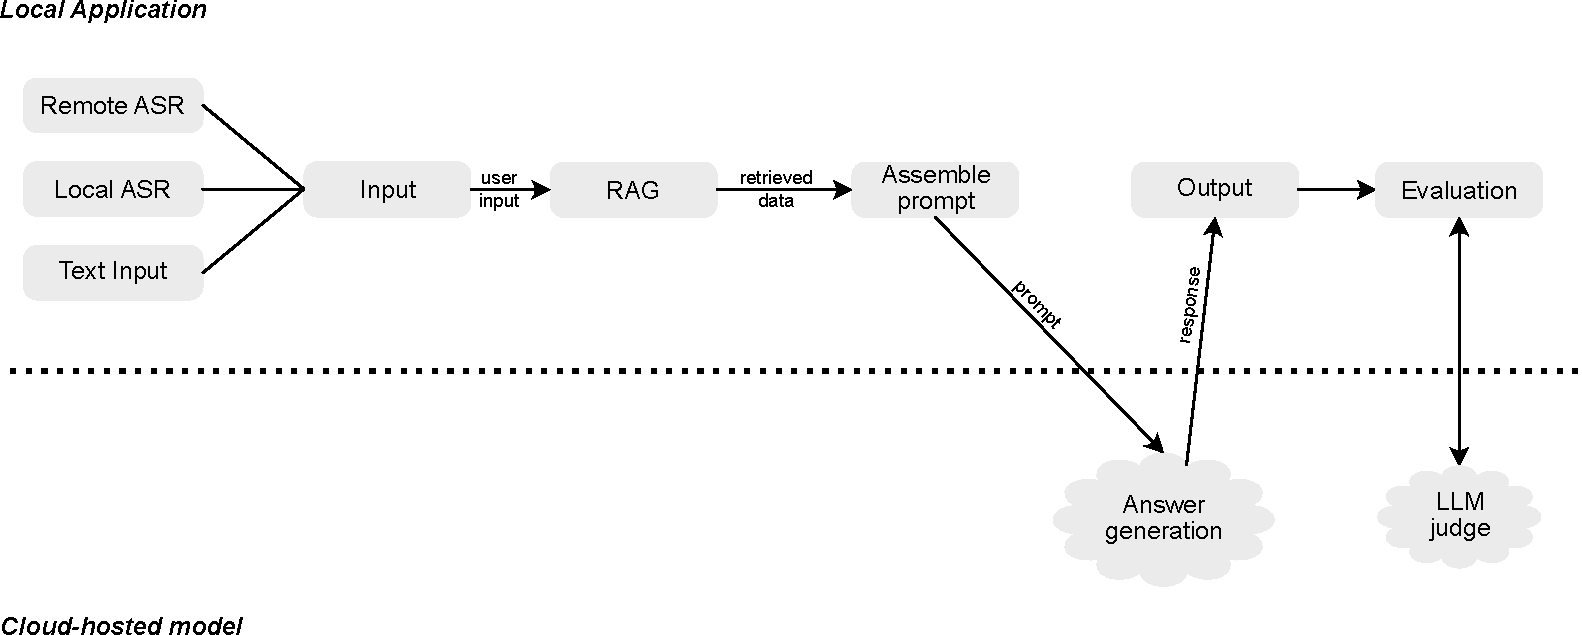
\includegraphics[width=1.0\linewidth]{images/data_flow_basic.pdf}
    \end{figure}
\end{frame}

\section{Data Flow Improvements}
\subsection{Identified Problems}
\begin{frame}{Identified Problems}
    \begin{itemize}
        \item ASR errors
            \begin{itemize}
                \item High impact on retrieval
                \item Especially building IDs (e.g. "Gebäude fünfzig Punkt zwanzig")
            \end{itemize}
        \item Missing multi-turn context
            \begin{itemize}
                \item Some queries rely on context
                \item No successful retrieval possible
                \item Model has to attend to conversation history
            \end{itemize}
        \item Inaccurate retrieval
            \begin{itemize}
                \item Embeddings unfit for matching numerical IDs
            \end{itemize}
        \item Too much returned information
            \begin{itemize}
                \item Model tends to use all provided data
                \item Unnecessary information in response
            \end{itemize}
        \item Suboptimal system prompt
            \begin{itemize}
                \item Language mismatch
                \item Low structure
                \item Instruction order
            \end{itemize}
    \end{itemize}
\end{frame}

\subsection{Implemented Solutions}
\begin{frame}[t]{Implemented Solutions}
    \vspace{-0.5cm}
	\begin{figure}
	    \centering
	    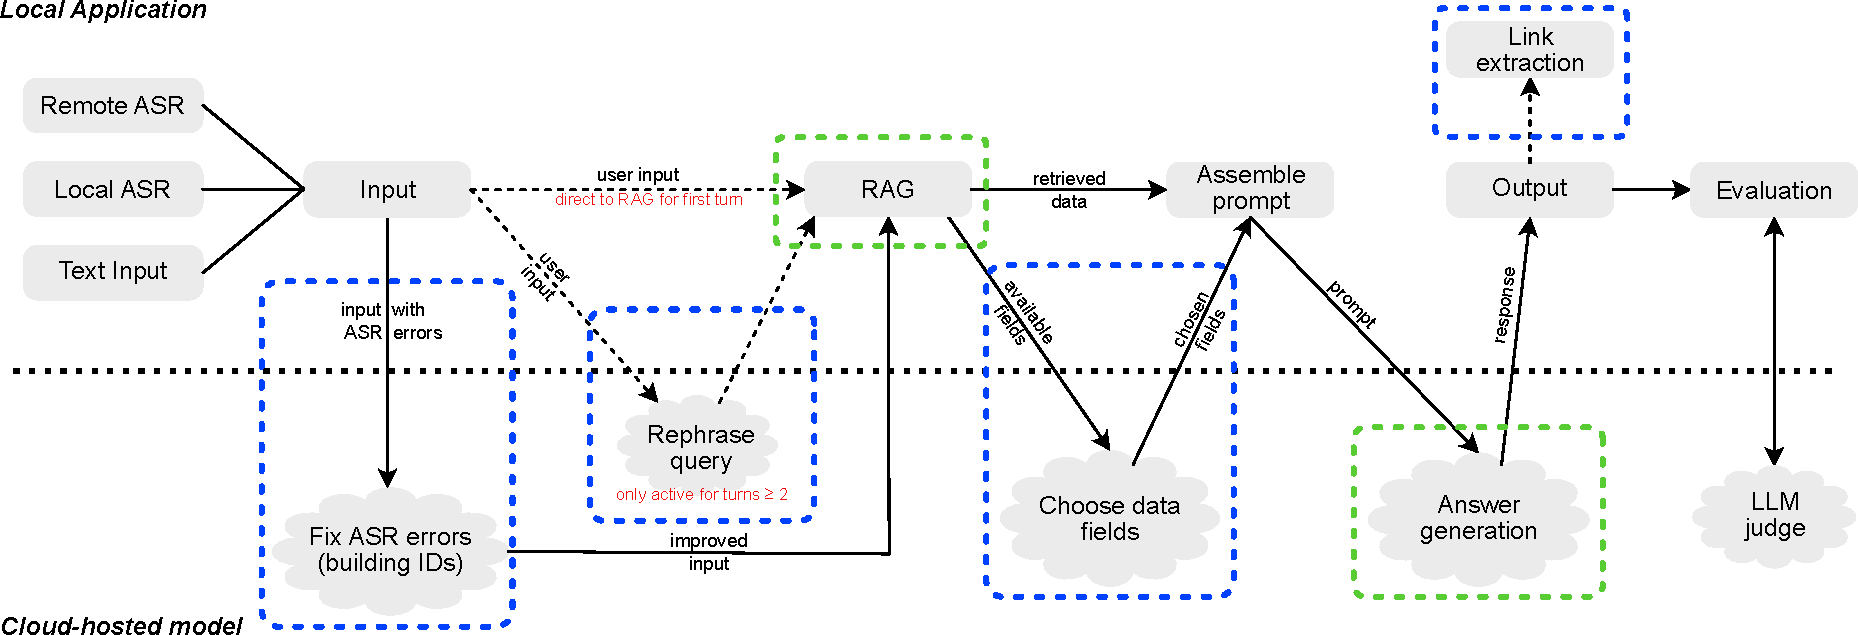
\includegraphics[width=1.0\linewidth]{images/data_flow_phase_3.pdf}
	\end{figure}
\end{frame}

\subsection{Final Evaluation}
\begin{frame}[t]{LLM Judge Score}
	\vspace{-1.5cm}
	\begin{figure}
	    \centering
	    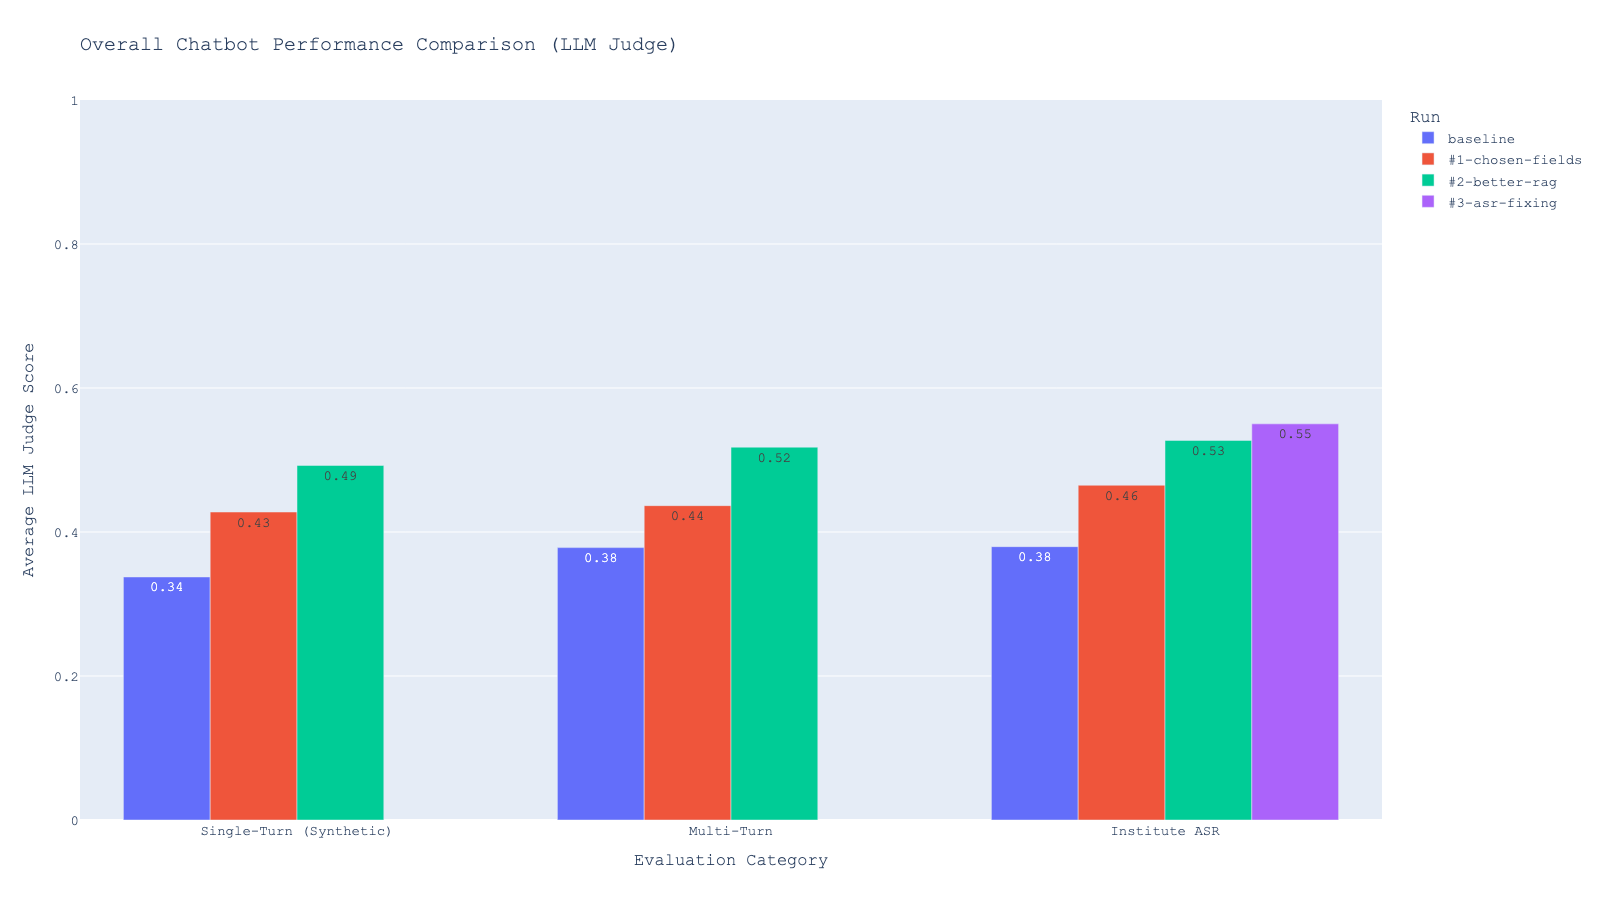
\includegraphics[width=0.75\linewidth]{images/overall_performance_comparison.png}
	\end{figure}
\end{frame}

\begin{frame}[t]{LLM Judge Score}
	\vspace{-1.5cm}
	\begin{figure}
	    \centering
	    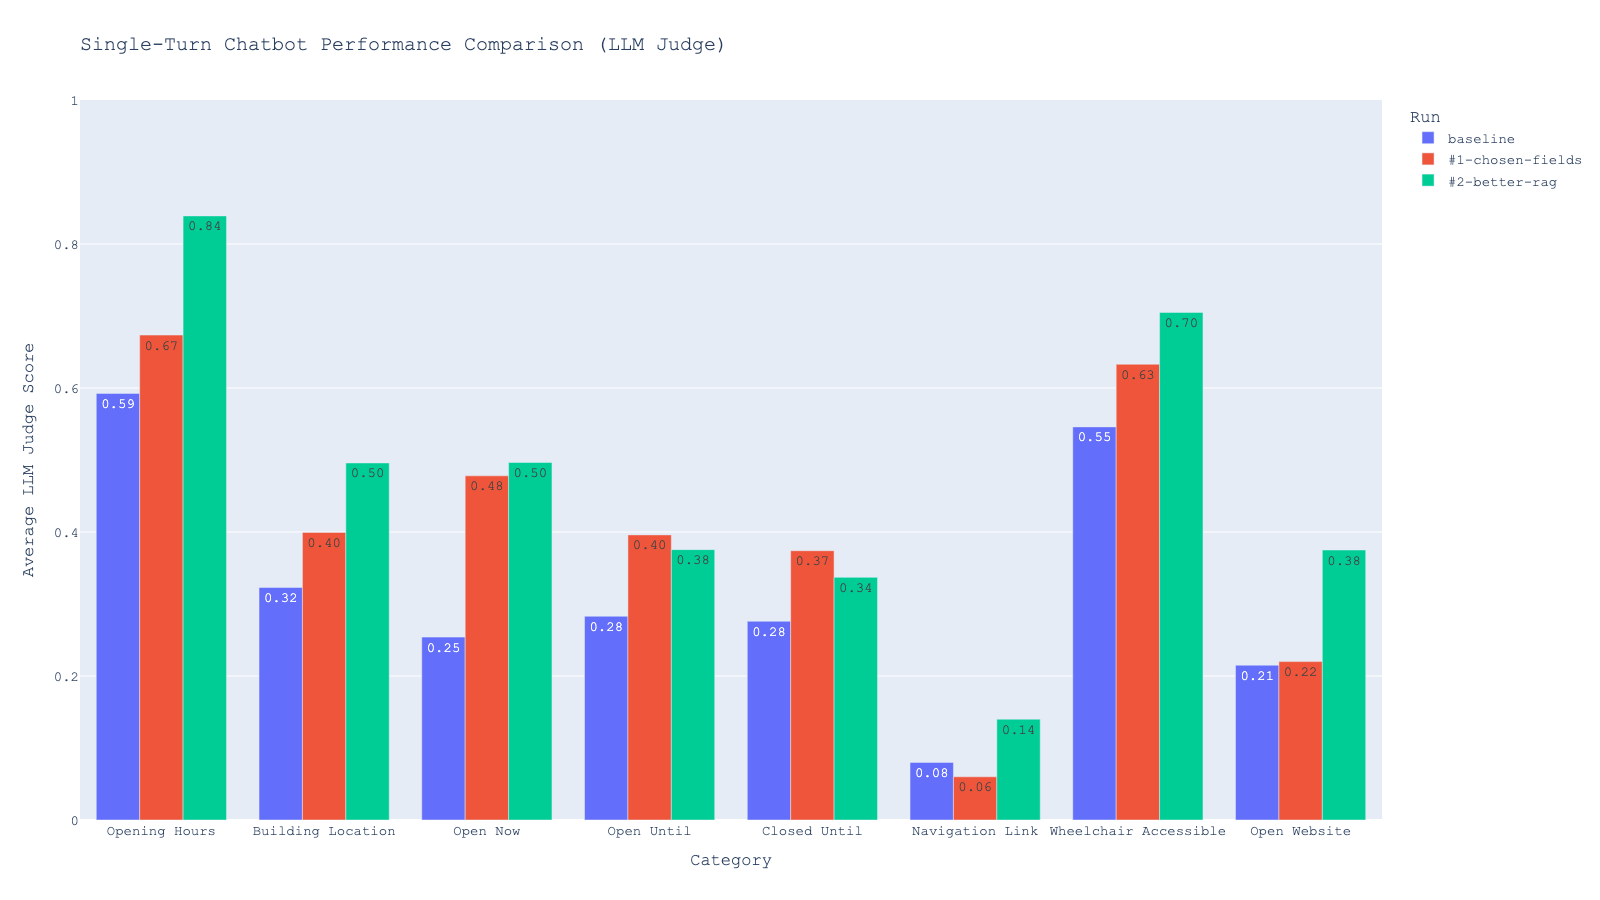
\includegraphics[width=0.75\linewidth]{images/single_turn_performance_comparison.png}
	\end{figure}
\end{frame}

\begin{frame}[t]{Pass/Fail Score}
\begin{table}[H]
    \centering
        \begin{tabular}{|l|c|c|c|c|}
        \hline
        \textbf{Category} & \textbf{\# Test Cases} & \textbf{Baseline} & \textbf{Improvements} \\
        \hline
        Building Location     & 85  & 19  & 40 \\
        Closed Until          & 100 & 24  & 31 \\
        Navigation Link       & 50  & 0   & 0  \\
        Open Now              & 100 & 20  & 45 \\
        Open Until            & 100 & 21  & 33 \\
        Open Website          & 100 & 17  & 34 \\
        Opening Hours         & 100 & 53  & 81 \\
        Wheelchair Accessible & 100 & 49  & 68 \\
        \hline
    \end{tabular}
\end{table}
\end{frame}

\section{Demo}
\begin{frame}{}
    \vspace{1.5cm}
    \centering
    \fontsize{100pt}{55pt}\selectfont \textcolor{kit-green100}{\textbf{Demo Time}}
\end{frame}


% \begin{frame}{Blöcke}{in den KIT-Farben}
% 	\begin{columns}
% 		\column{\kittwocolumns}
% 		\begin{greenblock}{Greenblock}
% 			Standard (\texttt{block})
%         \end{greenblock}
% 		\column{\kittwocolumns}
% 		\begin{royalblueblock}{Royalblueblock}
% 			= \texttt{exampleblock}
%         \end{royalblueblock}
% 		\column{\kittwocolumns}
% 		\begin{redblock}{Redblock}
% 			= \texttt{alertblock}
%         \end{redblock}
% 	\end{columns}
% 	\begin{columns}
% 		\column{\kittwocolumns}
% 		\begin{grayblock}{Grayblock}
% 			Text
%         \end{grayblock}
% 		\column{\kittwocolumns}
% 		\begin{lightgrayblock}{Lightgrayblock}
% 			Text
%         \end{lightgrayblock}
% 		\column{\kittwocolumns}
% 		\begin{blueblock}{Blueblock}
% 			Text
%         \end{blueblock}
% 	\end{columns}
% 	\begin{columns}
% 		\column{\kittwocolumns}
%         \begin{brownblock}{Brownblock}
% 			Text
%         \end{brownblock}
% 		\column{\kittwocolumns}
%         \begin{purpleblock}{Purpleblock}
% 			Text
%         \end{purpleblock}
% 		\column{\kittwocolumns}
%         \begin{cyanblock}{Cyanblock}
% 			Text
%         \end{cyanblock}
% 	\end{columns}
% 	\begin{columns}
% 		\column{\kittwocolumns}
%         \begin{yellowblock}{Yellowblock}
% 			Text
%         \end{yellowblock}
% 		\column{\kittwocolumns}
%         \begin{lightgreenblock}{Lightgreenblock}
% 			Text
%         \end{lightgreenblock}
% 		\column{\kittwocolumns}
%         \begin{orangeblock}{Orangeblock}
% 			Text
%         \end{orangeblock}
% 	\end{columns}
% 	\begin{columns}
% 		\column{\kittwocolumns}
% 		\begin{contentblock}{Contentblock}
% 			(farblos)
% 		\end{contentblock}
% 		\column{\kittwocolumns}
% 		\column{\kittwocolumns}
% 	\end{columns}
% \end{frame}

% \begin{frame}{Auflistungen}
% 	Text
% 	\begin{itemize}
% 		\item Auflistung\\ Umbruch
% 		\item Auflistung
% 		\begin{itemize}
% 			\item Auflistung
% 			\item Auflistung
% 		\end{itemize}
% 	\end{itemize}
% 	\begin{enumerate}
% 		\item Aufzählung
% 		\item Aufzählung
% 		\item Aufzählung
% 	\end{enumerate}
% \end{frame}

% \begin{frame}{Spalten}
% 	\begin{columns}
% 		\column{\kitcolumn}
% 		\begin{standardbox}
% 			Ich bin ein Blindtext.
% 		\end{standardbox}
% 		\column{\kitcolumn}
% 		\begin{highlightbox}
% 			Ich bin ein Blindtext.
% 		\end{highlightbox}
% 		\column{\kitcolumn}
% 		\begin{grayhighlightbox}
% 			Ich bin ein Blindtext.
% 		\end{grayhighlightbox}
% 		\column{\kitcolumn}
% 		\begin{lightgrayhighlightbox}
% 			Ich bin ein Blindtext.
% 		\end{lightgrayhighlightbox}
% 		\column{\kitcolumn}
% 		\begin{standardbox}
% 			Ich bin ein Blindtext.
% 		\end{standardbox}
% 		\column{\kitcolumn}
% 		\begin{standardbox}
% 			Ich bin ein Blindtext.
% 		\end{standardbox}
% 	\end{columns}
% 	\vspace{1em}
% 	\begin{columns}
% 		\column{\kittwocolumns}
% 		\begin{standardbox}
% 			Ich bin ein Blindtext.
% 		\end{standardbox}
% 		\column{\kittwocolumns}
% 		\begin{highlightbox}
% 			Ich bin ein Blindtext.
% 		\end{highlightbox}
% 		\column{\kittwocolumns}
% 		\begin{grayhighlightbox}
% 			Ich bin ein Blindtext.
% 		\end{grayhighlightbox}
% 	\end{columns}
% 	\vspace{1em}
% 	\begin{columns}
% 		\column{\kitthreecolumns}
% 		\begin{standardbox}
% 			Ich bin ein Blindtext.
% 		\end{standardbox}
% 		\column{\kitthreecolumns}
% 		\begin{highlightbox}
% 			Ich bin ein Blindtext.
% 		\end{highlightbox}
% 	\end{columns}
% \end{frame}

% \begin{frame}{Spalten}
% 	\begin{columns}
% 		\column{\kitfourcolumns}
% 			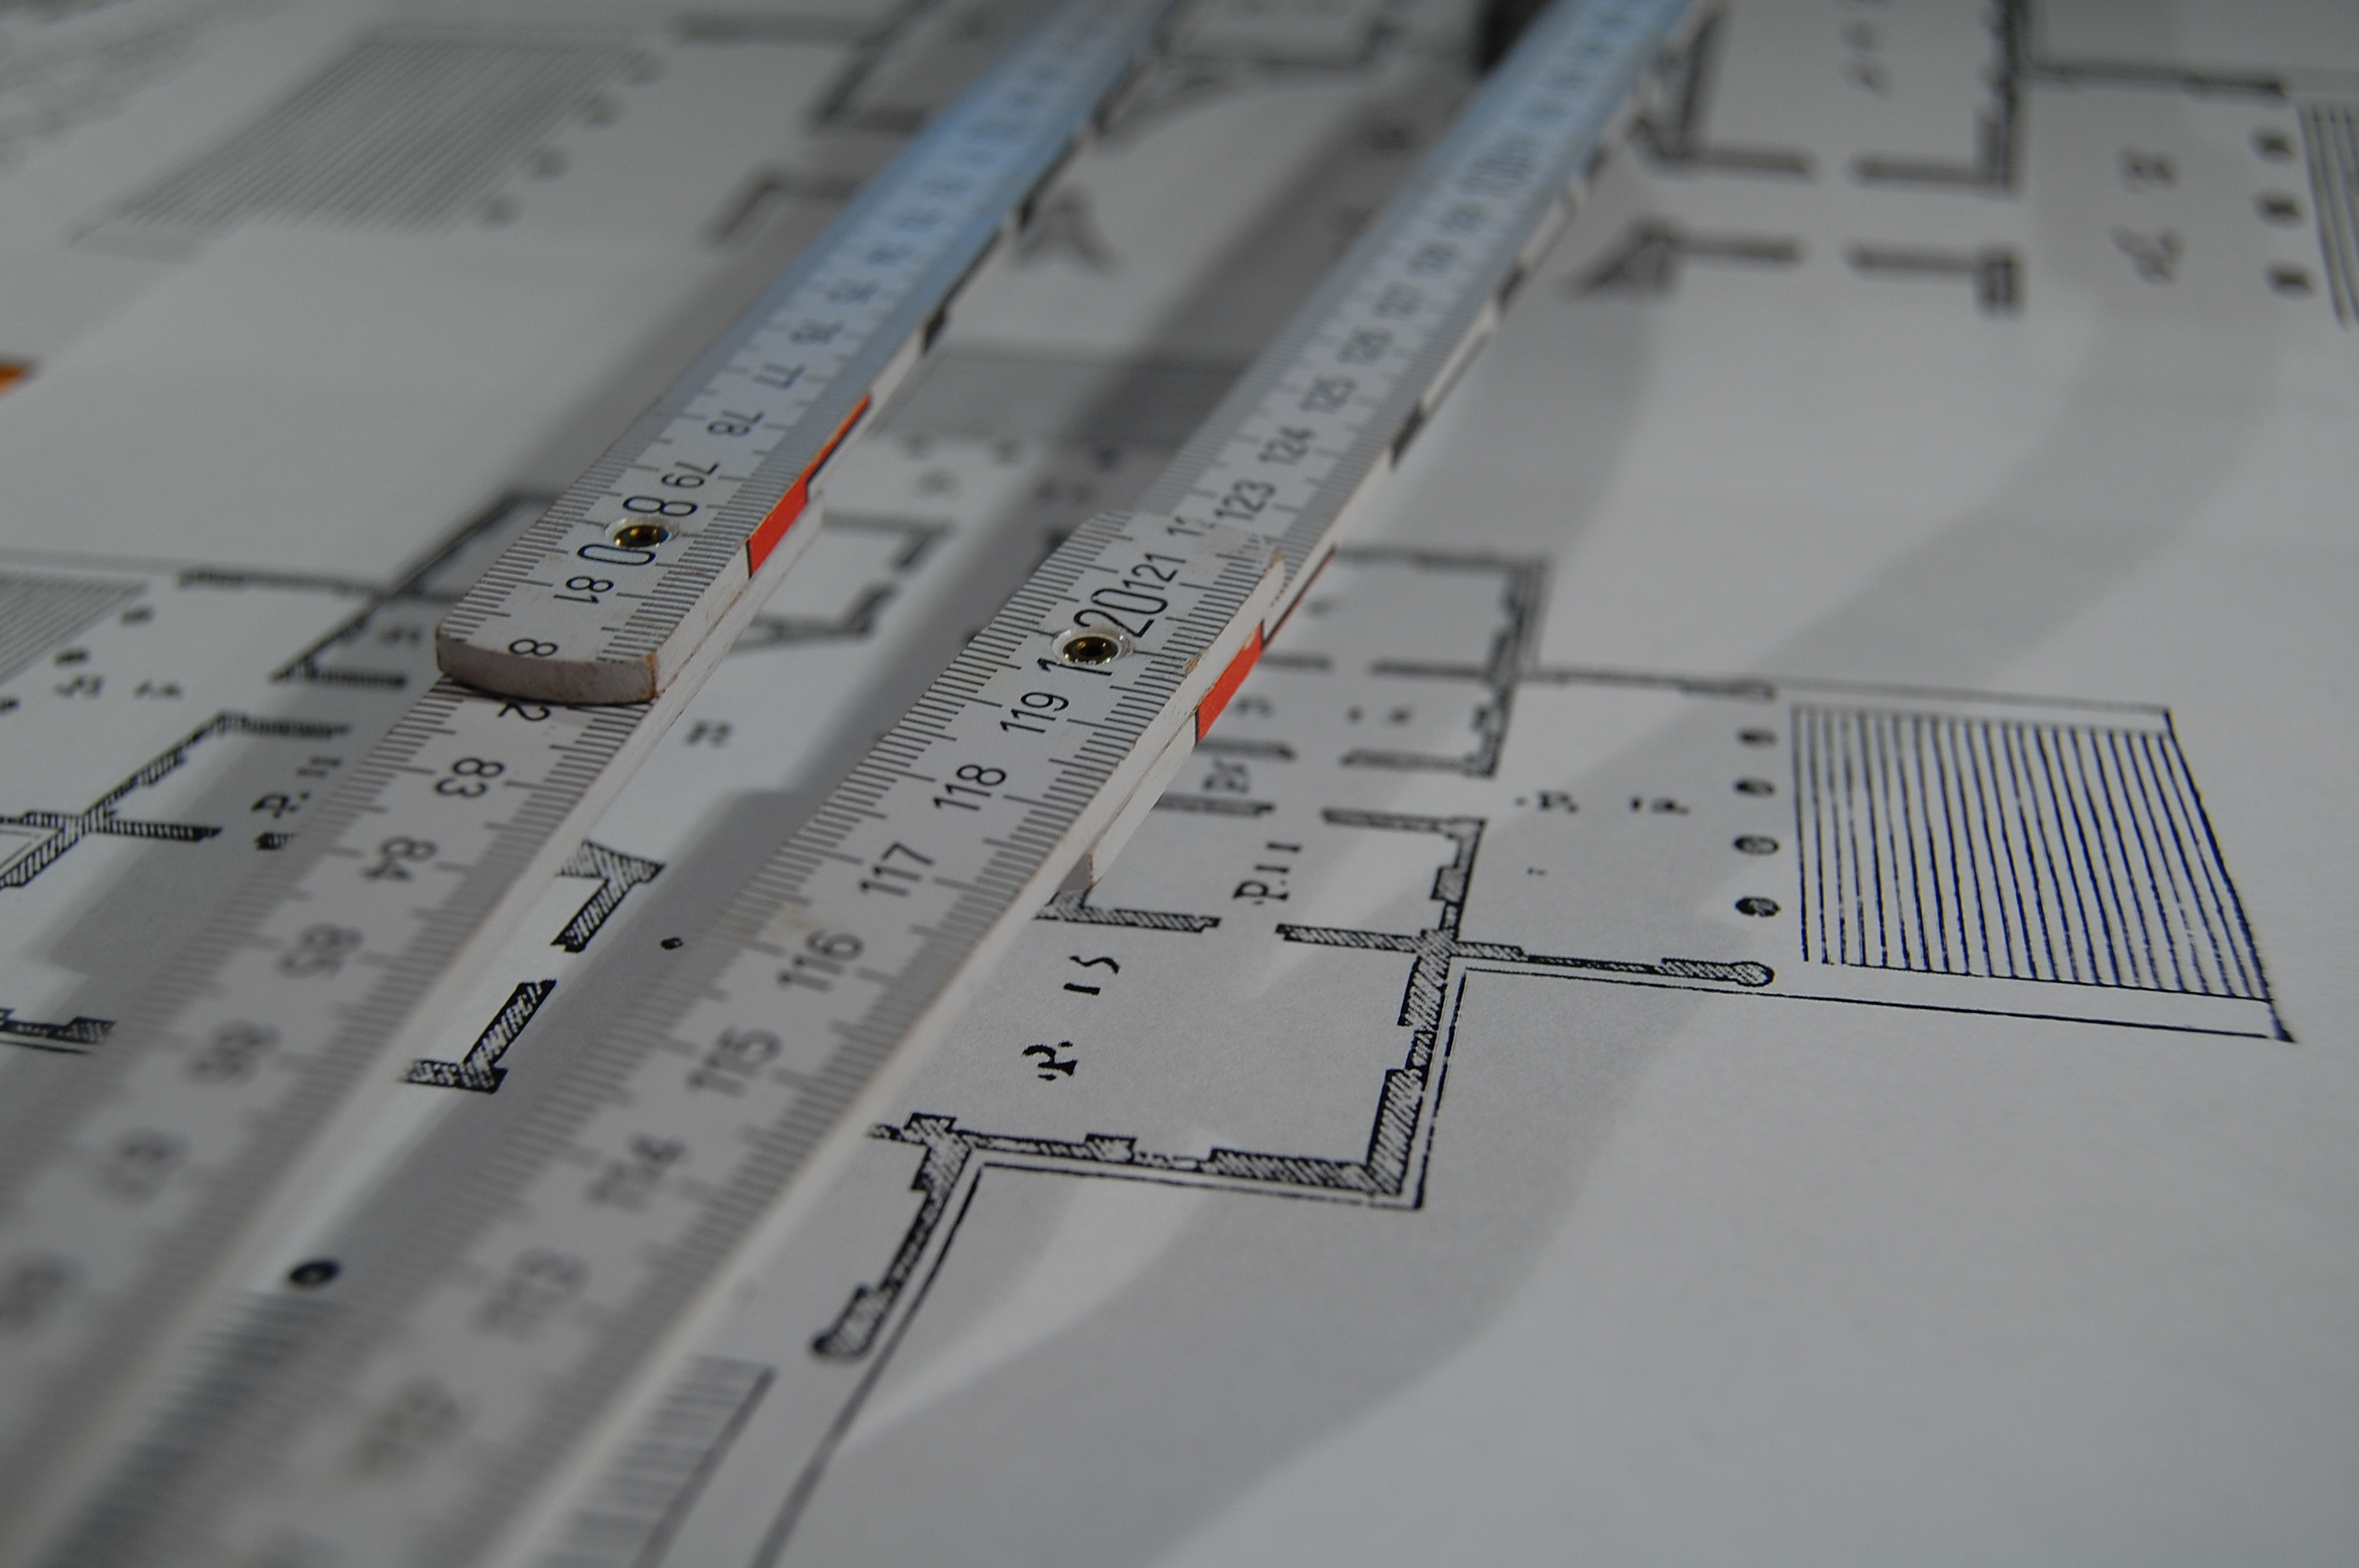
\includegraphics[width=\linewidth, trim={0 2cm 0 2cm}, clip]{images/palladio_bauplan.jpg}
% 		\column{\kittwocolumns}
% 			\begin{standardbox}
% 				Beschreibung
% 			\end{standardbox}

% 			\vspace{1em}

% 			\begin{highlightbox}
% 				Dies ist ein Bauplan der berühmten Villa Rotonda.
% 			\end{highlightbox}

% 			\vspace{1em}

% 			\begin{grayhighlightbox}
% 				Foto: Klaus Krogmann
% 			\end{grayhighlightbox}
% 	\end{columns}
% \end{frame}

% \begin{frame}[picture 66 vertical,picture=images/palladio_bauplan,kitlogo=black]{Folie mit Bild auf $\frac{2}{3}$ Größe}
% 	\lipsum[1][1-8]
% \end{frame}

% \begin{frame}[picture 50 vertical,picture=images/palladio_bauplan,kitlogo=black]{Folie mit Bild auf halber Größe}
% 	\lipsum[1][1-16]
% \end{frame}

% \begin{frame}[picture 33 vertical,picture=images/palladio_bauplan,kitlogo=white]{Folie mit Bild auf $\frac{1}{3}$ Größe}
% 	\begin{columns}
% 		\column{\kittwocolumns}
% 		\lipsum[1][1-8]
% 		\column{\kittwocolumns}
% 		\lipsum[1][1-8]
% 	\end{columns}
% \end{frame}


% \begin{frame}[picture vertical=20,picture=images/palladio_bauplan,kitlogo=white]{Folie mit Bild auf variabler Größe (20 \%)}
% 	\lipsum[1][1-16]
% \end{frame}


% \begin{frame}
%         Bei Frames ohne Titel wird die Kopfzeile nicht angezeigt, und
%     der freie Platz kann für Inhalte genutzt werden.
% \end{frame}

% \begin{frame}[plain]
%     Bei Frames mit Option \texttt{[plain]} werden weder Kopf- noch Fußzeile angezeigt.
% \end{frame}

% \begin{frame}[t]{Beispielinhalt}
%     Bei Frames mit Option \texttt{[t]} werden die Inhalte nicht vertikal zentriert, sondern an der Oberkante begonnen.
% \end{frame}

% \appendix
% \beginbackup

% \section{Farben}
% %% ----------------------------------------
% %% | Test-Folie mit definierten Farben |
% %% ----------------------------------------
% \begin{frame}{Farbpalette}
% \newcommand{\csq}{\strut\hskip1.2em}
% \begin{tabular}{rccccccccccccc}
% 	& 100 & 90 & 80 & 70 & 60 & 50 & 40 & 30 & 25 & 20 & 15 & 10 & 5\\
% % GREEN
% 	kit-green
% 	& \colorbox{kit-green100}{\csq}
% 	& \colorbox{kit-green90}{\csq}
% 	& \colorbox{kit-green80}{\csq}
% 	& \colorbox{kit-green70}{\csq}
% 	& \colorbox{kit-green60}{\csq}
% 	& \colorbox{kit-green50}{\csq}
% 	& \colorbox{kit-green40}{\csq}
% 	& \colorbox{kit-green30}{\csq}
% 	& \colorbox{kit-green25}{\csq}
% 	& \colorbox{kit-green20}{\csq}
% 	& \colorbox{kit-green15}{\csq}
% 	& \colorbox{kit-green10}{\csq}
% 	& \colorbox{kit-green5}{\csq}\\[.5em]
% % BLUE
% 	kit-royalblue
% 	& \colorbox{kit-royalblue100}{\csq}
% 	& \colorbox{kit-royalblue90}{\csq}
% 	& \colorbox{kit-royalblue80}{\csq}
% 	& \colorbox{kit-royalblue70}{\csq}
% 	& \colorbox{kit-royalblue60}{\csq}
% 	& \colorbox{kit-royalblue50}{\csq}
% 	& \colorbox{kit-royalblue40}{\csq}
% 	& \colorbox{kit-royalblue30}{\csq}
% 	& \colorbox{kit-royalblue25}{\csq}
% 	& \colorbox{kit-royalblue20}{\csq}
% 	& \colorbox{kit-royalblue15}{\csq}
% 	& \colorbox{kit-royalblue10}{\csq}
% 	& \colorbox{kit-royalblue5}{\csq}\\[.5em]
% % BLUE
% 	kit-blue
% 	& \colorbox{kit-blue100}{\csq}
% 	& \colorbox{kit-blue90}{\csq}
% 	& \colorbox{kit-blue80}{\csq}
% 	& \colorbox{kit-blue70}{\csq}
% 	& \colorbox{kit-blue60}{\csq}
% 	& \colorbox{kit-blue50}{\csq}
% 	& \colorbox{kit-blue40}{\csq}
% 	& \colorbox{kit-blue30}{\csq}
% 	& \colorbox{kit-blue25}{\csq}
% 	& \colorbox{kit-blue20}{\csq}
% 	& \colorbox{kit-blue15}{\csq}
% 	& \colorbox{kit-blue10}{\csq}
% 	& \colorbox{kit-blue5}{\csq}\\[.5em]
% % RED
% 	kit-red
% 	& \colorbox{kit-red100}{\csq}
% 	& \colorbox{kit-red90}{\csq}
% 	& \colorbox{kit-red80}{\csq}
% 	& \colorbox{kit-red70}{\csq}
% 	& \colorbox{kit-red60}{\csq}
% 	& \colorbox{kit-red50}{\csq}
% 	& \colorbox{kit-red40}{\csq}
% 	& \colorbox{kit-red30}{\csq}
% 	& \colorbox{kit-red25}{\csq}
% 	& \colorbox{kit-red20}{\csq}
% 	& \colorbox{kit-red15}{\csq}
% 	& \colorbox{kit-red10}{\csq}
% 	& \colorbox{kit-red5}{\csq}\\[.5em]
% % GREY
% 	kit-gray
% 	& \colorbox{kit-gray100}{\csq}
% 	& \colorbox{kit-gray90}{\csq}
% 	& \colorbox{kit-gray80}{\csq}
% 	& \colorbox{kit-gray70}{\csq}
% 	& \colorbox{kit-gray60}{\csq}
% 	& \colorbox{kit-gray50}{\csq}
% 	& \colorbox{kit-gray40}{\csq}
% 	& \colorbox{kit-gray30}{\csq}
% 	& \colorbox{kit-gray25}{\csq}
% 	& \colorbox{kit-gray20}{\csq}
% 	& \colorbox{kit-gray15}{\csq}
% 	& \colorbox{kit-gray10}{\csq}
% 	& \colorbox{kit-gray5}{\csq}\\[.5em]
% % Orange
% 	kit-orange
% 	& \colorbox{kit-orange100}{\csq}
% 	& \colorbox{kit-orange90}{\csq}
% 	& \colorbox{kit-orange80}{\csq}
% 	& \colorbox{kit-orange70}{\csq}
% 	& \colorbox{kit-orange60}{\csq}
% 	& \colorbox{kit-orange50}{\csq}
% 	& \colorbox{kit-orange40}{\csq}
% 	& \colorbox{kit-orange30}{\csq}
% 	& \colorbox{kit-orange25}{\csq}
% 	& \colorbox{kit-orange20}{\csq}
% 	& \colorbox{kit-orange15}{\csq}
% 	& \colorbox{kit-orange10}{\csq}
% 	& \colorbox{kit-orange5}{\csq}\\[.5em]
% % lightgreen
% 	kit-lightgreen
% 	& \colorbox{kit-lightgreen100}{\csq}
% 	& \colorbox{kit-lightgreen90}{\csq}
% 	& \colorbox{kit-lightgreen80}{\csq}
% 	& \colorbox{kit-lightgreen70}{\csq}
% 	& \colorbox{kit-lightgreen60}{\csq}
% 	& \colorbox{kit-lightgreen50}{\csq}
% 	& \colorbox{kit-lightgreen40}{\csq}
% 	& \colorbox{kit-lightgreen30}{\csq}
% 	& \colorbox{kit-lightgreen25}{\csq}
% 	& \colorbox{kit-lightgreen20}{\csq}
% 	& \colorbox{kit-lightgreen15}{\csq}
% 	& \colorbox{kit-lightgreen10}{\csq}
% 	& \colorbox{kit-lightgreen5}{\csq}\\[.5em]
% % Brown
% 	kit-brown
% 	& \colorbox{kit-brown100}{\csq}
% 	& \colorbox{kit-brown90}{\csq}
% 	& \colorbox{kit-brown80}{\csq}
% 	& \colorbox{kit-brown70}{\csq}
% 	& \colorbox{kit-brown60}{\csq}
% 	& \colorbox{kit-brown50}{\csq}
% 	& \colorbox{kit-brown40}{\csq}
% 	& \colorbox{kit-brown30}{\csq}
% 	& \colorbox{kit-brown25}{\csq}
% 	& \colorbox{kit-brown20}{\csq}
% 	& \colorbox{kit-brown15}{\csq}
% 	& \colorbox{kit-brown10}{\csq}
% 	& \colorbox{kit-brown5}{\csq}\\[.5em]
% % Purple
% 	kit-purple
% 	& \colorbox{kit-purple100}{\csq}
% 	& \colorbox{kit-purple90}{\csq}
% 	& \colorbox{kit-purple80}{\csq}
% 	& \colorbox{kit-purple70}{\csq}
% 	& \colorbox{kit-purple60}{\csq}
% 	& \colorbox{kit-purple50}{\csq}
% 	& \colorbox{kit-purple40}{\csq}
% 	& \colorbox{kit-purple30}{\csq}
% 	& \colorbox{kit-purple25}{\csq}
% 	& \colorbox{kit-purple20}{\csq}
% 	& \colorbox{kit-purple15}{\csq}
% 	& \colorbox{kit-purple10}{\csq}
% 	& \colorbox{kit-purple5}{\csq}\\[.5em]
% % Cyan
% 	kit-cyan
% 	& \colorbox{kit-cyan100}{\csq}
% 	& \colorbox{kit-cyan90}{\csq}
% 	& \colorbox{kit-cyan80}{\csq}
% 	& \colorbox{kit-cyan70}{\csq}
% 	& \colorbox{kit-cyan60}{\csq}
% 	& \colorbox{kit-cyan50}{\csq}
% 	& \colorbox{kit-cyan40}{\csq}
% 	& \colorbox{kit-cyan30}{\csq}
% 	& \colorbox{kit-cyan25}{\csq}
% 	& \colorbox{kit-cyan20}{\csq}
% 	& \colorbox{kit-cyan15}{\csq}
% 	& \colorbox{kit-cyan10}{\csq}
% 	& \colorbox{kit-cyan5}{\csq}\\[.5em]
% \end{tabular}
% \end{frame}
% %% ----------------------------------------
% %% | /Test-Folie mit definierten Farben |
% %% ----------------------------------------
% \backupend

\end{document}
